\section*{2.5 Newton varias variables}

En esta sección se utilizará una extensión del método de Newton para aproximar la solución al problema solo que esta vez los conceptos y herramientas del calculo serán en varias variables. Con afán de hacer lo más sencillo posible el cambio de una variable a varias variables se realizarán comparaciones geométricas entre éstas dos. 

\subsection*{Funciones de varias variables}
Primero: pensemos en una función cuya representación geométrica es una parábola figura \ref{tab:funcion}


\begin{figure*}[h!]
\centering
  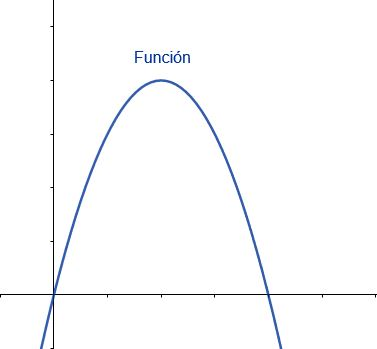
\includegraphics[width=0.4\textwidth]{funcion1.JPG}
\caption{Parábola}
\label{tab:funcion}
\end{figure*} 

Ahora pensemos que rotamos la parábola en torno a la linea que se forma de unir el vértice con el foco, esto provocará que la gráfica deje de estar en el plano y ahora se convierta en un objeto conocido como paraboloide: figura \ref{tab:fun3}.

\begin{figure*}[h!]
\centering
  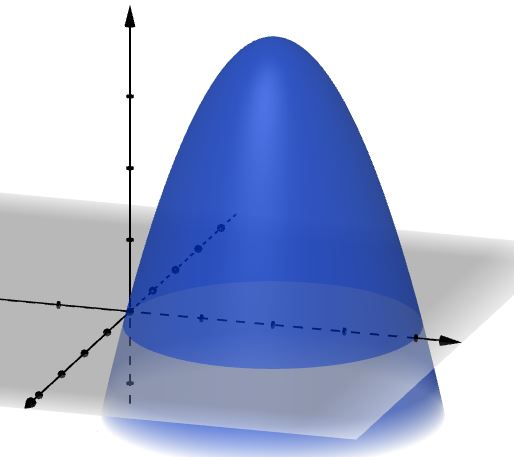
\includegraphics[width=0.45\textwidth]{funcion2.JPG}
\caption{Paraboloide}
\label{tab:fun3}
\end{figure*} 

Pues bien, como se podrá intuir, las funciones de varias variables $f(x,y,z,...)$ son la generalización de las funciones de una variable $f(x)$ con las cuales estamos más familiarizados, esto quiere decir que ahora ya no solo dependerá de una variable sino de dos o más y que, dependiendo del plano con el cual ``toquemos'' a la función de varias variables nos dará distintas funciones (proyecciones) en dicho plano.

\subsection*{Derivada en varias variables}
Ahora recordemos que la representación geométrica de la derivada es la \textbf{recta tangente} de la función $f(x)=y$, en otras palabras, es la recta que interseca a la función en un solo punto y si la evaluamos nos indica cual es el valor de la pendiente en dicho punto. 

En las figuras \ref{tab:fig6}, \ref{tab:fig7} y \ref{tab:fig8} se ilustra como es que la recta se va ``moviendo'' por la gráfica hasta solo tocar en un punto donde es la recta de interés. 

\begin{multicols}{3}
\begin{figure}[H]
\centering
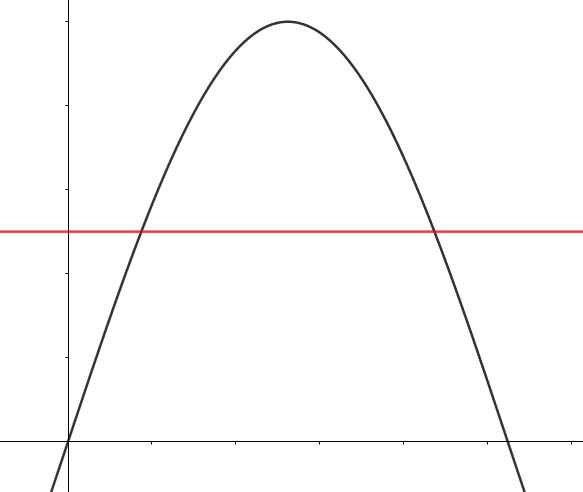
\includegraphics [ width =0.3\textwidth ]{aprox1.jpg}
\caption{Cuerda}
\label{tab:fig6}
\end{figure}
\begin{figure}[H]
\centering
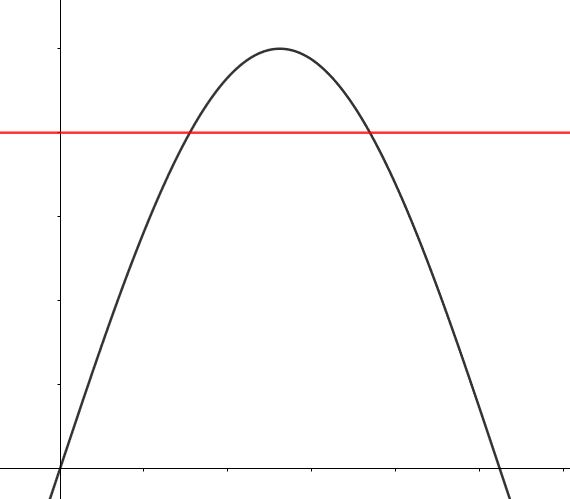
\includegraphics [ width =0.3\textwidth ]{aprox2.JPG}
\caption{Secante}
\label{tab:fig7}
\end{figure}
\begin{figure}[H]
\centering
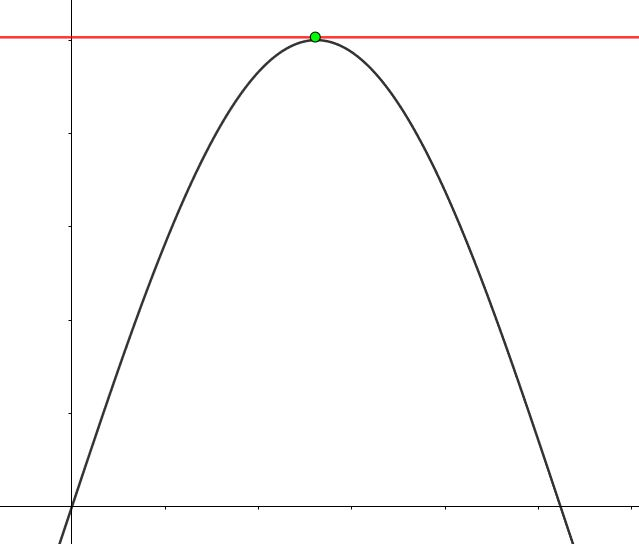
\includegraphics [ width =0.3\textwidth ]{aprox3.JPG}
\caption{\textbf{Tangente}}
\label{tab:fig8}
\end{figure}
\end{multicols}

Es de esperarse que en funciones de varias variables se pueda derivar con respecto a las variables que aparecen en la función y no solo una como anteriormente se hacía; por ejemplo si tenemos la función $f(x,y,z)=(f_1,f_2,f_3)=(2x^2yz,5xy^4z,3xyz^3)$ podremos \textbf{derivar parcialmente} con respecto a $x$, $y$ o $z$ entonces tendremos:

\begin{equation*}
    \frac{\partial}{\partial x} f(x,y,z)=\frac{\partial}{\partial x}(f_1,f_2,f_3)=(\frac{\partial}{\partial x} f_1,\frac{\partial}{\partial x} f_2,\frac{\partial}{\partial x} f_3)=(\frac{\partial}{\partial x} 2x^2yz,\frac{\partial}{\partial x} 5xy^4z,\frac{\partial}{\partial x} 3xyz^3)
\end{equation*}
Notemos que la derivada es respecto a $x$ por lo tanto todas las demás variables son constantes ante ésta y por ello ``salen'' de la derivada y queda:

\begin{equation*}
\begin{split}
    \frac{\partial}{\partial x} f(x,y,z)&=(2yz \frac{\partial}{\partial x}x^2,5y^4z\frac{\partial}{\partial x}x,3yz^3\frac{\partial}{\partial x}x)\\
    &=(2yz(2x),5y^4z(1),3yz^3(1))
\end{split}
\end{equation*}
Finalmente
\begin{equation*}
    \frac{\partial}{\partial x} f(x,y,z)=(4xyz,5y^4z,3yz^3)
\end{equation*}

Análogamente con las otras dos derivadas parciales pero ahora con $y$ y $z$:

\begin{equation*}
\begin{split}
    \frac{\partial}{\partial y} f(x,y,z)&=(2x^2z \frac{\partial}{\partial y}y,5xz\frac{\partial}{\partial y}y^4,3xz^3\frac{\partial}{\partial y}y)\\
    &=(2x^2z(1),5xz(4y^3),3xz^3(1))\\
    &=(2x^2z,20xy^3z,3xz^3)
\end{split}
\end{equation*}

Y

\begin{equation*}
\begin{split}
    \frac{\partial}{\partial z} f(x,y,z)&=(2x^2y \frac{\partial}{\partial z}z,5xy^4\frac{\partial}{\partial z}z,3xy\frac{\partial}{\partial z}z^3)\\
    &=(2x^2y(1),5xy^4(1),3xy(3z^2))\\
    &=(2x^2y,5xy^4,9xyz^2)
\end{split}
\end{equation*}

Entonces tenemos los siguientes resultados:

\begin{equation*}
\begin{split}
    (\frac{\partial}{\partial x} f_1,\frac{\partial}{\partial x} f_2,\frac{\partial}{\partial x} f_3)&=(4xyz,5y^4z,3yz^3)\\
    (\frac{\partial}{\partial y} f_1,\frac{\partial}{\partial y} f_2,\frac{\partial}{\partial y} f_3)&=(2x^2z,20xy^3z,3xz^3)\\ 
    (\frac{\partial}{\partial z} f_1,\frac{\partial}{\partial z} f_2,\frac{\partial}{\partial z} f_3)&=(2x^2y,5xy^4,9xyz^2)
\end{split}
\end{equation*}

Que si lo escribimos de manera matricial es:

\begin{equation*}
\Large
\begin{pmatrix}
\frac{\partial f_1}{\partial x} & \frac{\partial f_2}{\partial x} & \frac{\partial f_3}{\partial x}\\
\frac{\partial f_1}{\partial y} & \frac{\partial f_2}{\partial y} & \frac{\partial f_3}{\partial y}\\
\frac{\partial f_1}{\partial z} & \frac{\partial f_2}{\partial z} & \frac{\partial f_3}{\partial z}
\end{pmatrix}
=
\begin{pmatrix}
4xyz & 5y^4z & 3yz^3\\
2x^2z & 20xy^3z & 3xz^3\\
2x^2y & 5xy^4 & 9xyz^2
\end{pmatrix}
\end{equation*} 

Pues bien, si transponemos la matriz (los vectores columna cambian a vectores fila o viceversa) queda de la forma:

\begin{equation*}
\Large
\begin{pmatrix}
\frac{\partial f_1}{\partial x} & \frac{\partial f_1}{\partial y} & \frac{\partial f_1}{\partial z}\\
\frac{\partial f_2}{\partial x} & \frac{\partial f_2}{\partial y} & \frac{\partial f_2}{\partial z}\\
\frac{\partial f_3}{\partial x} & \frac{\partial f_3}{\partial y} & \frac{\partial f_3}{\partial z}
\end{pmatrix}
=
\begin{pmatrix}
4xyz & 2x^2z & 2x^2y\\
5y^4z & 20xy^3z & 5xy^4\\
3yz^3 & 3xz^3 & 9xyz^2
\end{pmatrix}
\end{equation*} 

Y lo que acabamos de obtener se le conoce como \textbf{la matriz jacobiana} que será de suma importancia en el tema que nos compete.

Cabe resaltar que se puede dar el caso de tener una función general con $m$ componentes $(f_1,f_2,\dotso,f_m)$ y dependiente de $n$ variables $f(x_1,x_2,\dotso,x_n)$, en dicho caso la matriz jacobiana es no necesariamente cuadrada y se escribe de la forma:

\begin{equation*}
\Large
\textbf{Matriz \ jacobiana \ general}\Rightarrow 
\begin{pmatrix}
\frac{\partial f_1}{\partial x_1} & \dotsb & \frac{\partial f_1}{\partial x_n}\\
\vdots & \ddots & \vdots\\
\frac{\partial f_m}{\partial x_1} & \dotsb & \frac{\partial f_m}{\partial x_n}
\end{pmatrix}
\end{equation*} 


\subsection*{Método de Newton en varias variables}
Ahora bien, retomemos la ecuación del método de Newton para una variable:

\begin{equation*}
    p_n= p_{n-1} -\frac{f(p_{n-1})}{f'(p_{n-1})}, \ para \ n\geq 1.
\end{equation*}

Primero hay que notar que la función depende una sola variable $p_{n-1}$ y también el punto de partida guarda información sólo de la variable $x$ puesto que $p_0=x_0$; ahora bien, el propósito de todo lo anterior fue dar las bases para la generalización del método y es muy natural pensar que, al tener una \textbf{función de varias variables} todos los demás elementos sean también en varias variables como se muestra en la tabla \ref{tab:tabla7}.

\begin{table}[h!]
\centering
    \begin{tabular}{||c c c||}
    \hline 
    \hline
        \multicolumn{3}{c}{\textbf{Generalización}}\tabularnewline
        Una variable &  & Varias variables (dependiente de $x,y$) \\
    \hline 
    \hline 
        $f(p_{n-1})$ & $\rightarrow$ & \textbf{Función} \\
        $f'(p_{n-1})$ & $\rightarrow$ & $\textbf{Jacobiano de f}$ \\
        $p_n$  & $\rightarrow$ & \textbf{Vector $p_n$} \\
        $p_{n-1}$ & $\rightarrow$ & \textbf{Vector $p_{n-1}$} \\
        \hline
        \hline 
    \end{tabular}
\caption{Una variable - varias variables}
\label{tab:tabla7} 
\end{table}

Nota: en la literatura al \textbf{jacobiano de f} se puede encontrar como \textbf{$J_f$}, D\textbf{f} o $ \nabla\textbf{f} $. 

Entonces la ecuación para el método de Newton en varias variables es:

\begin{equation*}
    \textbf{p}_n= \textbf{p}_{n-1} -[\nabla\textbf{f}(p_{n-1})]^{-1} \textbf{f}(p_{n-1}), \ para \ n\geq 1.
\end{equation*}

Cuyo proceso es descrito por el algoritmo de \textbf{Newton en varias variables}

\begin{tcolorbox}[colback=blue!15!]
\subsubsection*{Newton en varias variables}
Para encontrar la solución a $\textbf{f}(x,y)=0$ dada la aproximación inicial $\textbf{p}_0$:
\\ \\
ENTRADA aproximación inicial $p_0$; tolerancia \textit{TOL}; número máximo de iteraciones $N_0$.

SALIDA La solución aproximada \textit{p} o mensaje de falla.

PASO 1 Asigna i=1;

PASO 2 Mientras $i\leq N_0$ ejecuta los pasos 3-6.

\ \ \ \  PASO 3 Asigna $\textbf{p}=\textbf{p}_0 -[\nabla\textbf{f}(\textbf{p}_0)]^{-1} \textbf{f}(\textbf{p}_0) $; (calcula $p_i$)

\ \ \ \  PASO 4 Si $||\textbf{p}-\textbf{p}_0||<TOL$ entonces

\ \ \ \ \ \ \ \ \ \ \ \ \ \ \ \ \ \ SALIDA (p); (proceso completado exitosamente)

\ \ \ \ \ \ \ \ \ \ \ \ \ \ \ \ \ \ ALTO.

\ \ \ \   PASO 5 Asigna $i=i+1$
    
\ \ \ \   PASO 6 Asigna $\textbf{p}_0=\textbf{p}$; (Actualiza $p_0$.)

PASO 7 SALIDA ('El método fallo después de $N_0$ iteraciones $N_0=$',$N_0$);

\ \ \ \ \ \ \ \ \ \ \ \ \ (El proceso fue exitoso.)

\ \ \ \ \ \ \ \ \ \ \ \ \ ALTO.


\end{tcolorbox}